\section{Implementation}
	\subsection{Sprint 0}
		\subsubsection{Sprint Planning}
		As the initial one of the project, this sprint was concerned with setting up and configuring CI/CD tools for the project. The main tool of the CI/CD process considered was a Jenkins build server to continuously build and deploy the code. Given the agile development methodology it was important to implement these steps early in the project and therefore they were undertaken during the initial sprint.

		\subsubsection{Sprint Review}
		The following goals were achieved:
		\begin{itemize}
			\item A Jenkins build server was deployed to AWS;
			\item An AWS ECS instance to run the web app was deployed;
			\item A skeleton React app was created with a defined Dockerfile to build image of the app;
			\item A Jenkins pipeline was created to build the image of the app and deploy it to AWS on every commit to GitHub;
		\end{itemize}
		
		\subsubsection{Sprint Retrospective}
		\textbf{What did we do well?}
		\begin{itemize}	
			\item CI/CD process has been set-up and implemented.
		\end{itemize}
		
		\noindent\textbf{What could have been done better?}
		\begin{itemize}
			\item Story Points have not been allocated to tickets;
			\item Breakdown of backlog could be improved, better utilising Epics, Issues and Subtasks.
		\end{itemize}
		
		\noindent\textbf{Actions}
		\begin{itemize}
			\item Rob Shelly to further refine the product backlog;
			\item Rob Shelly to add story points to tickets on backlog.
		\end{itemize}
		
		\subsubsection{Personal Reflection}
		This sprint highlighted the need for story points as the lack of such has meant there is not burndown chart for the sprint. Adding story points along with a well refined and organised backlog will allow for better sprint planning in the future.

	\subsection{Sprint 1}
		\subsubsection{Sprint Planning}
		The planning for this sprint was based on the existing Jenkins Jobs created during the prototyping process. These jobs need to exist on the Jenkins server when the system is initially deployed/installed by a user. i.e, the user does not create these jobs.
		Therefore, these jobs need to be created during the installation process. This sprint focused on creating \textit{yaml} files for these jobs which can be used by \textit{Jenkins Job Builder} (JJB) to create the jobs during set-up. This also provided the ability to quickly recreate the jobs should the Jenkins Server crash during development.

		\subsubsection{Sprint Review}
		The \textit{yaml} files were created and tested for the following Jenkins jobs:
		\begin{itemize}
			\item Deploy: Spins up a restoration server in AWS (i.e. a server with the correct DBMS installed)
			\item Decrypt:  Moves a backup file to a restoration server and decrypts it.
			\item Restore: Imports a backup file into the DBMS and performs a read of the data.
			\item Destroy: Destroys the restoration server after a successful backup restoration.
			\item Backup Restoration Pipeline:	Performs a full backup test restoration (using the above Jenkins jobs).
		\end{itemize}
		The sprint delivered on its main goal of creating the \textit{yaml} files. However, further tickets which would have built upon the prototype (displaying the result of the restoration) were not completed.

		\subsubsection{Sprint Retrospective}
		\textbf{What did we do well?}
		\begin{itemize}	
			\item Technically mastered the complexity of the project, have a
			vision and a direction to move towards;
			\item Backlog is very mature, the Minimum Viable Product (MVP) is almost visible;
			\item JJB was utilised and I now understand how Jenkins jobs
			work;
			\item Story Points were introduced and helped to guide the work.
		\end{itemize}
		
		\noindent\textbf{What could have been done better?}
		\begin{itemize}
			\item Burndown was inconsistent as most of the work was completed within a short period of time during the sprint;
			\item Domain knowledge in certain areas (JJB) was not as strong
			as I would have liked it to be, which slowed me down and
			was not reflective of the complexity I had awarded those
			tickets;
			\item Outward communication to the stakeholders (Leigh \& Paul)
			was not as good as it could have been.
		\end{itemize}

		\noindent\textbf{Actions}
		\begin{itemize}
			\item Rob Shelly to get a draft of wireframes to Leigh by next Monday;
			\item Rob Shelly to complete MVP plan for the backend system and include an API definition and CLI guide;
      \item Rob Shelly to send regular updates on progress to stakeholders.
		\end{itemize}

		\subsubsection{Sprint Burndown}
		
 		\begin{figure}[H]
      \setlength{\belowcaptionskip}{15pt plus 3pt minus 2pt}
      \caption{Sprint 1 Burndown Chart}
      \centering
      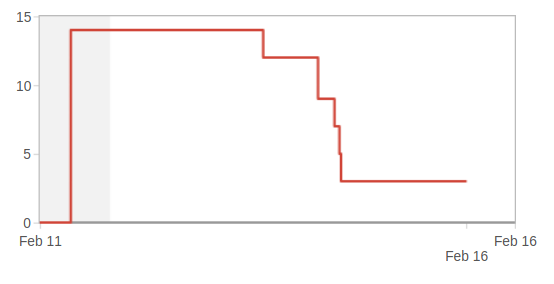
\includegraphics[width=\textwidth,keepaspectratio]{burndown-sprint-1}
      \label{fig:burndown-sprint-1}
    \end{figure}
   
		\subsubsection{Personal Reflection}
		I was happy with the progress of this sprint as I felt creating the \textit{yaml} files for the Jenkins jobs was a vital task, not only to enable an MVP to be packaged as a deployable system, but also to provide an easy method of recreating the Jenkins jobs should there be a loss of AWS servers during development.
		
		This sprint also highlighted the importance of planning the sprint with respect to other college work to be completed in the given time frame. Although, this sprint was planned for two weeks, the entirety of the work was completed within a number of days during the later of two weeks. In future, if other college work will take precedence for a number of days, I may plan to delay beginning the sprint, allowing the final burndown chart to better reflect the progress of work over the sprint.
    
  \subsection{Sprint 2}
  \subsubsection{Sprint Planning}
  Planning for this sprint focused on completing the API for my systems. Through conversations with the stakeholders it was decided that the priority for this sprint should be completing the API and its documentation. Creating the web app frontend for the API could be completed later. However, given that there was still quite a larger number of API related tickets on the product backlog, not all were brought into this sprint.
  
  \subsubsection{Sprint Review}
  The following API function were implemented:
  \begin{itemize}
    \item Get results of all recent test restoration;
    \item Get a list of all scheduled test restorations;
    \item Create a new test restoration schedule;
    \item Update test restoration schedule;
    \item Delete a test restorations schedule;
    \item Get results of all test restorations for a given schedule;
    \item Add an SSH key to the system;
    \item Add a GPG key to the system.
  \end{itemize}
  Documentation for each of the API functions was also completed using Swagger Docs. Thus, the sprint delivered on it's goal of completing and documenting the bulk of the API functions.
  
  \subsubsection{Sprint Retrospective}
  \textbf{What did we do well?}
  \begin{itemize}
    \item Working on a concentrated area (API) was very beneficial;
    \item Product owners were satisfied with the increase in progress updates;
    \item A lot of knowledge was gained around the documentation using Swagger,  helping to develop the backend without the need for a frontend to test it;
    \item Time management was better than the previous sprint, results on all tickets being completed.
  \end{itemize}
  
  \noindent\textbf{What could have been done better?}
  \begin{itemize}
    \item Burndown chart, although better than the previous sprint is still somewhat inconsistent. However, with all tickets completed, the overall result is still good.
  \end{itemize}
  
  \noindent\textbf{Actions}
  \begin{itemize}
    \item Rob Shelly to complete the last few API related tickets from the backlog in order to allows work to proceed to focus solely on the UI.
  \end{itemize}
  
  \subsubsection{Sprint Burndown}
  
  \begin{figure}[H]
    \setlength{\belowcaptionskip}{15pt plus 3pt minus 2pt}
    \caption{Sprint 2 Burndown Chart}
    \centering
    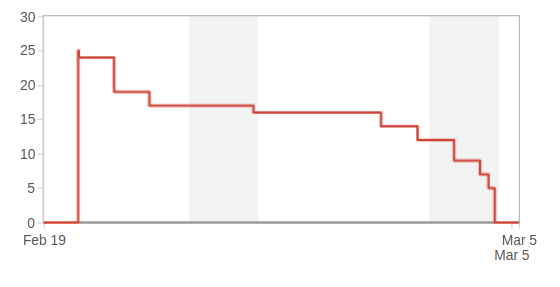
\includegraphics[width=\textwidth,keepaspectratio]{burndown-sprint-2}
    \label{fig:burndown-sprint-2}
  \end{figure}
  
  \subsubsection{Personal Reflection}
  I was very happy with the work completed during this sprint. Prior to Sprint planning and backlog refinement I had been planning on completing tickets by grouping API functions with their corresponding UI elements. However, on the advice of the product owners I decided to focus solely on completing the API first before moving on to the UI.
  
  Having completed the sprint I now feel that separating the API and UI was a much more productive approach. Swagger, which was used to document the API also contains a feature to test the the documented API calls. Therefore, by focusing only on writing and documenting the API, I was able to stay in the mindset of the API functions without having to constantly transition between developing API calls and UI elements, while still being able to test the functions using Swagger.
  
   \subsection{Sprint 3}
   \subsubsection{Sprint Planning}
   Planning for this sprint focused on two main areas the first of the which was to finalise the backend API. The plan set out with the product owners prior to the previous sprint dictated that the backend API should be completed before focusing on the UI. Therefore, in accordance with the actions dictated during the previous retrospective, finishing the last remaining tickets concerning the API would be the initial focus of this sprint.
   
   Given that there was only a small number of API related tickets remaining on the backlog, the second aspect of this sprint was beginning work on the UI. Accordingly. a number of user 
   
   \subsubsection{Sprint Review}
   The sprint achieved it's goal by completing the final API related tickets and implementing the first features of the UI. The following API functions were completed:
   \begin{itemize} 
     \item API function to list all SSH keys;
     \item API function to list all GPG keys;
     \item API function to delete an SSH key;
     \item API function to delete a GPG key.
   \end{itemize}
   Additionally, the following UI elements were created:
  \begin{itemize} 
    \item A web form to run a single backup restoration;
    \item A page displaying the results of recent backup restorations;
    \item A web form to schedule regular backup restorations.
  \end{itemize}
  
  \subsubsection{Sprint Retrospective}
  \textbf{What did we do well?}
  \begin{itemize}
   \item Having completed all the backend API calls, the MVP was clearly defined;
   \item Time was better managed than in previous sprints, having chosen to delay the start of the sprint while working on other projects;
   \item Burndown chart was consistent and reflective of better time management.
  \end{itemize}
   
   \noindent\textbf{What could have been done better?}
   \begin{itemize}
     \item Communication with the product owners was bad due to time spent on other projects;
     \item UI design highlighted an issue with the API leading to some refactoring.
   \end{itemize}
   
   \noindent\textbf{Actions}
   \begin{itemize}
     \item Rob Shelly to decide if a Command Line Interface (CLI) should be implemented.
   \end{itemize}
   
   \subsubsection{Sprint Burndown}
   
   \begin{figure}[H]
     \setlength{\belowcaptionskip}{15pt plus 3pt minus 2pt}
     \caption{Sprint 3 Burndown Chart}
     \centering
     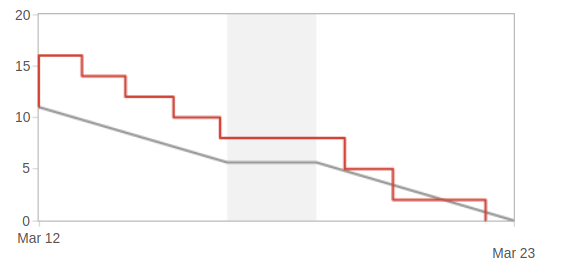
\includegraphics[width=\textwidth,keepaspectratio]{burndown-sprint-3}
     \label{fig:burndown-sprint-3}
   \end{figure}
   
   \subsubsection{Personal Reflection}
   I was happy to complete the backend during this sprint, allowing time to begin working on the UI without need to worry about the underlying API calls. This reinforced benefit of product owners recommendation to complete the API before beginning the UI. However, beginning work on the UI did highlight an issue with the backend. During UI work I realised that I had not created one of the necessary function calls. Although it was a simple solution to create the API call when needed, the time needed to do so was a setback on UI work.
   
   I felt my time management was much better during this sprint. Previous sprints featured periods of inactivity due to time spent on other projects. This was indicated by inconsistent burndown charts. Therefore I chose to delay the start of this sprint while I worked on other projects. This allowed me to focus on this project for the duration of the sprint once it had commenced. This was reflected in a much more consistent burndown chart.
   
   During this sprints retrospective the product owners mentioned the possibility of creating a command line interface (CLI) for the system. A CLI would allow more advance users to use the system without the need to visit the UI. This is something the product owners have indicated is a common desire amongst more advanced users who are more comfortable using the command line. I was disappointed that this thought had not occurred to me during project planning. At this stage of development, undertaking such a task might not be feasible, or may detract from my ability to implement a satisfactory UI. I felt that my two options for an MVP were to either focus entirely on the UI or reduce some UI features and also implement a CLI. I decided with the product owners that I should make the decisions prior to commencing my next sprint.
   
   \subsection{Sprint 4}
   \subsubsection{Sprint Planning}
    Having completed work on the API during the previous sprint, this sprint focused heavily on creating the UI. During the planning phase of this sprint a decision was made to focus entirely on the UI for the purpose of creating an MVP and that a CLI would be implemented in a future version. Therefore, it was decided that the remaining UI related tickets should all be completed during this sprint.
   
   \subsubsection{Sprint Review}
   This sprint achieved its goal of finishing the remaining UI related tickets. The following UI elements were created:
   \begin{itemize}
     \item A web form to add SSH keys;
     \item A web form to remove SSH keys;
     \item A web form to add GPG keys;
     \item A web form to remove GPG keys;
     \item A web form to modify a scheduled restoration;
     \item A web page to display all schedules;
     \item A web page to display all results of a given schedule.
    \end{itemize}
    This sprint added to email notification function to the system.
    
    \subsubsection{Sprint Retrospective}
    \textbf{What did we do well?}
    \begin{itemize}
      \item Time management was good, resulting in a consistent burndown chart;
      \item A decision was made and justified regarding the implementation of a CLI;
      \item Communication with the product owners was good, including keeping them up to date on the decision to focus on the UI.
    \end{itemize}
    
    \noindent\textbf{What could have been done better?}
    \begin{itemize}
      \item Email notification system should have been implemented earlier;
      \item Implementation of the email system highlighted issues with system design.
    \end{itemize}
    
    \noindent\textbf{Actions}
    \begin{itemize}
      \item Rob Shelly to consider how to package final product.
    \end{itemize}
    
    \subsubsection{Sprint Burndown}
    
    \begin{figure}[H]
      \setlength{\belowcaptionskip}{15pt plus 3pt minus 2pt}
      \caption{Sprint 4 Burndown Chart}
      \centering
      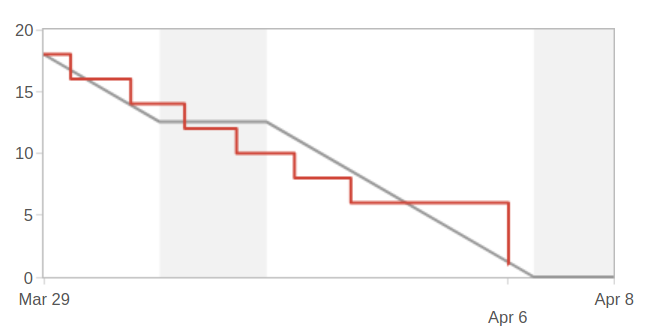
\includegraphics[width=\textwidth,keepaspectratio]{burndown-sprint-4}
      \label{fig:burndown-sprint-4}
    \end{figure}
    
    \subsubsection{Personal Reflection}
    I was very pleased with the result of this sprint having completed the UI work. At this point an MVP was almost complete. I was very happy that I had taken the product owner's advice to separate work on the backend and frontend. The benefits of this decision really showed during this sprint when I was able to focus almost exclusively on the UI, except for some minor refactoring.
    
    Prior to starting this sprint I made the decision to focus on implementing a comprehensive UI for the MVP, choosing to push the CLI to the backlog and implement it for a later version. Due to the limited time to complete this project I felt that I could not satisfactorily implement both a UI and CLI. The only option would have been to complete only basic user features for the UI and advanced user features for the CLI. However, I believe in order to deliver a useable and demonstrable system that at least one of the interfaces should be completed in its entirety. Thus, I made the decision to focus on the UI, which graphically emphasises the results of restorations.
   
    During this week I also completed work on the email notification system. In retrospect I should implemented this function earlier as notification of failed backups is a main objective of the system. Also, during the development of the function a flaw in the systems logic was noticed which may cause the system to fail to notify the users when a backup process has not succeeded. Although a fix was easily implemented, it would have been preferable to notice and overcome this issue earlier in development.
    
   In accordance with the actions listed during the previous retrospective, prior to commencing this sprint some consideration was given to packaging the final product. Previously the plan had been to package the UI as a Docker image, while the Jenkins backend would run on an AWS instance. This however would require some setup of the systems. Therefore, it was decided that if possible the system should be packaged entirely within a single Docker image.
   
	\subsection{Sprint 5}
  \subsubsection{Sprint Planning}
  Planning for this spring was concerned with delivering the MVP as a packaged product. During the previous sprint retrospective with the product owners, they suggested that the final product be packaged as a Docker image. However, after some research into this it was decided that the better solution would be to deliver two Docker images, one for the Jenkins management server and one for the UI web server. This in fact is a better practice as it is not advisable to run more than one service inside a Docker container. This will still allow the final product to be easily run as both containers will be able to communicate with one another.
  
  Prior to this sprint it was decided that although a fully implemented user system would be pushed to the backlog for development for a later version, it would be preferable to have at least a single \textit{admin} account to authenticate at the frontend. This would provide an extra layer of security allowing the web app to be deployed to a public domain without the system being exposed.
  
  \subsubsection{Sprint Review}
  This sprint achieved its goal of delivering a packaged MVP to the product owners. The following tickets were completed in order to package the system:
  
  \begin{itemize}
    \item Created a Dockerfile which defines the image of the UI;
    \item Created a Dockerfile which defines the image of the Jenkins server;
    \item Created XML definitions of all necessary Jenkins jobs to allow their creation during the image build process.
    \item Create Groovy script to configure Jenkins during the image build process including configuring jobs, security and the SMTP server for email.
  \end{itemize}
  
  \subsubsection{Sprint Retrospective}
  \textbf{What did we do well?}
  \begin{itemize}
    \item System was packed as easily runnable Docker images;
    \item An MVP was delivered to the product owners on schedule;
    \item Consideration was made for the security of the system and basic user authentication implemented as a result;
    \item Time management was good, reflected by a consistent burndown chart;
    \item Communication with products owners was good.
  \end{itemize}
  
  \subsubsection{Sprint Burndown}
  
  \begin{figure}[H]
    \setlength{\belowcaptionskip}{15pt plus 3pt minus 2pt}
    \caption{Sprint 5 Burndown Chart}
    \centering
    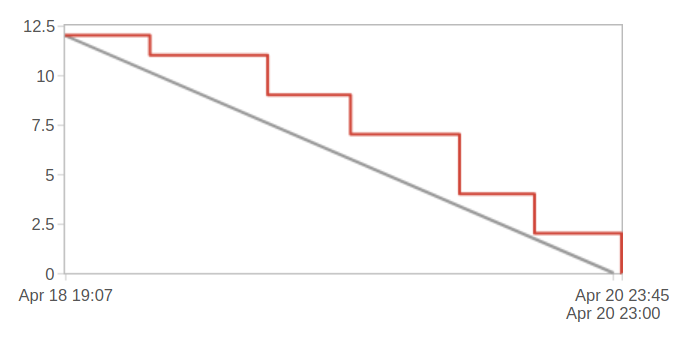
\includegraphics[width=\textwidth,keepaspectratio]{burndown-sprint-5}
    \label{fig:burndown-sprint-5}
  \end{figure}
  
  \subsubsection{Personal Reflection}
  I felt this was a very successful sprint as it not only delivered an MVP to the product owners but did so on schedule. I was very happy with the final product packaged as two Docker containers. During sprint planning I experimented with running two services inside a single container and found that although it was possible, it was quite unstable and often crashed. After reading Docker's supporting documentation I feel not only was the choice to implement two images a practical decision but also in keeping with best practices. The final MVP is also very stable in this configuration. 
  
  I was also very pleased to have been able to implement basic user authentication during this sprint. At previous sprint planning sessions and retrospectives it had been suggested that due to the current sprint velocities, authentication may need to be pushed to the backlog for development in a version succeeding the MVP. Although I felt this was a safe decision to make for an MVP as the system would quite possibly by to deployed as an internal service (i.e. within private networks), the addition of authentication certainly strengthens the security of the product.
  
  Overall I was quite happy with this sprint as I feel it was quite reflective of the lessons learned over previous sprints. Strong sprint planning meant that no refactoring or backtracking was needed as the right decision was made with regards to building one or two Docker images. This also helped time management and contributed to an ideal burndown of story points. 

	\subsection{Sprint Metrics}
  
  \subsection{Sprint Velocities}
  A Velocity Chart is shown in \autoref{fig:velocity}.  This shows the work committed to and completed in each of the sprints in terms of story points. The chart shows that initially the development time available during the sprints was being overestimated. Thus, in the first two sprints all tickets committed were not completed. However, by the third sprint this had been rectified, with better estimations and time management leading to  more consistent results.
  
  \begin{figure}[H]
    \setlength{\belowcaptionskip}{15pt plus 3pt minus 2pt}
    \caption{Velocity Chart}
    \centering
    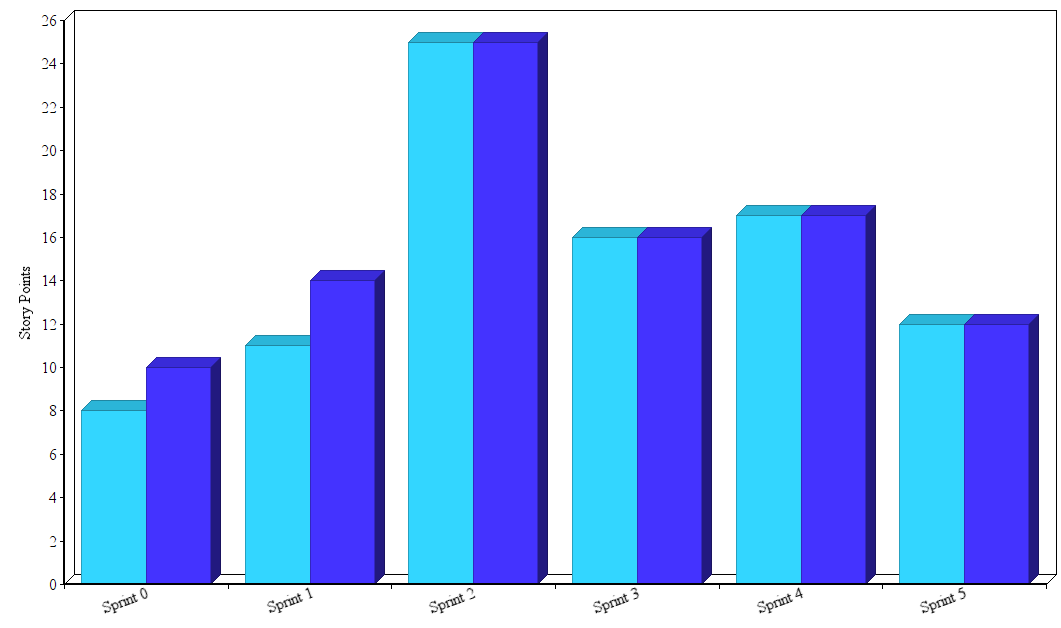
\includegraphics[width=\textwidth,keepaspectratio]{velocity}
    \label{fig:velocity}
  \end{figure}

	\subsection{Sprint Burndowns}
  Sprint burndown charts have been provided for completed sprints. The burndown charts provided valuable feedback on the development of each sprint. This is especially evident from earlier sprints where the charts highlighted that much of the development work was begin carried out during a relatively short period of the two-week-long sprints. This was due to time also spent on other projects. This feedback helped to better manage time in subsequent sprints in which they may have been delayed or shortened to reflected only the time allocated to this project.